%PHẦN CỦA KHOA
\newpage
\subsection{Module 5: Tìm kiếm và lọc kết quả; Đặt phòng homestay}

\subsubsection{ Tìm kiếm và lọc homestay}
\begin{figure}[!h]
	\centering
	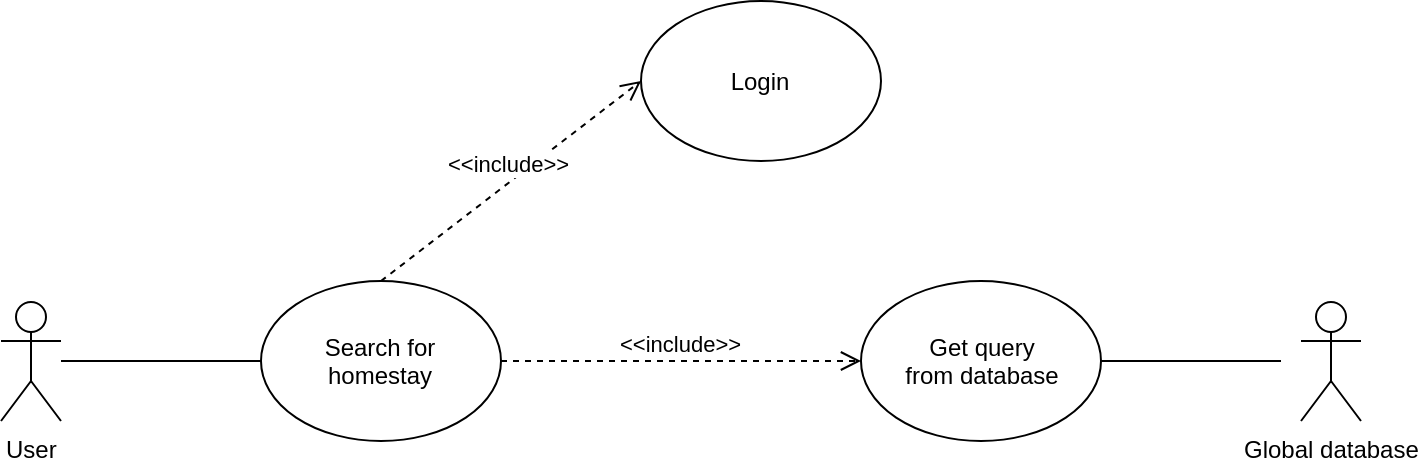
\includegraphics[width = 10cm, height = 4cm]{parts/Khoa/khoa_ui/search.png}
	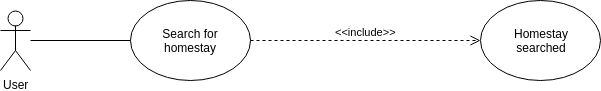
\includegraphics[width = 10cm, height = 1cm]{parts/Khoa/khoa_ui/filter.png}
	\caption{Lược đồ use case của Module 5: Tìm kiếm và lọc kết quả;}
\end{figure}
\begin{figure}[!h]
	\centering
	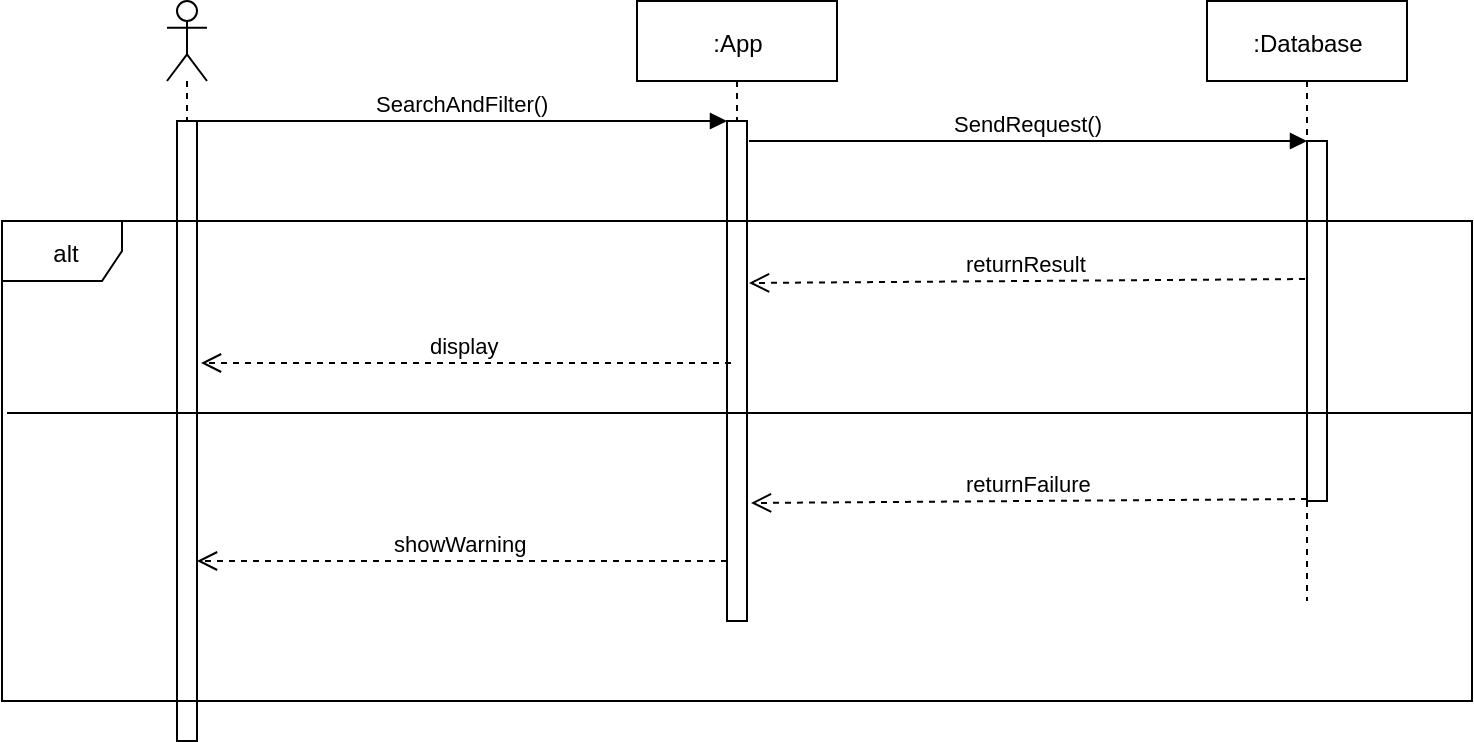
\includegraphics[width = 10cm, height = 6cm]{parts/Khoa/khoa_ui/khoa_search_and_filter.png}
	\caption{Sequence diagram của Module 5: Tìm kiếm và lọc kết quả;}
\end{figure}
\subsubsubsection{User Story}
Một trong những chức năng cơ bản và quan trọng nhất của trang web tìm kiếm homestay chính là chức năng tìm kiếm và lọc kết quả cho người dùng. Người dùng sẽ cung cấp một số thông tin cho ứng dụng, bao gồm địa điểm, vị trí. Sau đó, nếu người dùng có sử dụng thêm tính năng lọc, thì người dùng sẽ cung cấp các thông tin khác như rating yêu cầu của homestay, yêu cầu người dùng,... Sau khi thông tin được cung cấp, ứng dụng sẽ rà soát các homestay tại địa điểm, vị trí mà người dùng cung cấp. Ngoài ra, nếu người dùng có sử dụng tính năng lọc, danh sách các homestay được rà soát trên sẽ được lọc theo tiêu chí của người dùng. Kết quả cuối cùng sẽ là danh sách kết quả các homestay mà người dùng muốn tìm kiếm.
 \\
\subsubsubsection{Mô tả các use case}
\begin{enumerate}[label=\textbf{(\alph*)}]
	\item \textbf{Usecase 1: Tìm kiếm kết quả.}
	\begin{center}
		\begin{longtable}{ | l |p{10cm}|}
			\hline
			\textbf{Tên usecase} & TÌm kiếm kết quả homestay. \\ \hline
			\textbf{Người tương tác} & Người dùng ứng dụng. \\ \hline   
			\textbf{Mô tả} &  Người dùng tìm kiếm homestay dựa theo tên địa điểm.\\ \hline  
			\textbf{Người tạo:} \textit{Nguyễn Phan Đăng Khoa} & \textbf{Cập nhật lần cuối bởi:} \textit{Nguyễn Phan Đăng Khoa} \\ \hline
			\textbf{Ngày tạo:} \textit{22/03/2019} & \textbf{Lần cuối cập nhật:} \textit{30/03/2019} \\ \hline
			\textbf{Tiền điều kiện} &  Trước khi có thể sử dụng chức năng tìm kiếm, người dùng phải đăng nhập vào trang web. \\ \hline 
			\textbf{Hậu điều kiện} &  Danh sách các homestay mà người muốn tìm kiếm được hiển thị rõ ràng trên ứng dụng. \\ \hline 
			\textbf{Luồng cơ bản} & 
			\begin{enumerate}
				\item Người dùng chọn vào khung tìm kiếm và gõ vào vị trí/ tên homestay cần tìm.
				\item Người dùng chọn ngày "Check in", ngày "Check out" và số lượng khách đi.
				\item Người dùng nhấn chọn nút "Tìm kiếm"/Enter.
				\item Hệ thống hiển thị danh sách các tin chưa được duyệt, đang đợi duyệt.
				\item Danh sách các homestay, cùng với giá tiền, rating,... sẽ được thể hiện rõ ràng trên trang chính của trang web.
			\end{enumerate} \\ \hline 
			\textbf{Luồng thay thế} & 
			\begin{itemize} 
				\item \textit{Luồng thay thế 1}
				\begin{enumerate}
					\item Tại bước 4: Nếu không tìm thấy homestay thỏa điều kiện, trang web có thể hiện thông báo "Không tìm thấy".
				\end{enumerate}
			\end{itemize} \\ \hline 
			\textbf{Ngoại lệ}  & Không có \\
			\hline
		\end{longtable}
	\end{center}
\end{enumerate}

\begin{enumerate}[label=\textbf{(\alph*)}]
	\item \textbf{Usecase 2: Lọc kết quả đã tìm kiếm}
	\begin{center}
		\begin{longtable}{ | l |p{10cm}|}
			\hline
			\textbf{Tên usecase} & Lọc kết quả \\ \hline
			\textbf{Người tương tác} & Người dùng ứng dụng \\ \hline   
			\textbf{Mô tả} & Người dùng lọc homestay mà mình đã tìm kiếm. \\ \hline  
			\textbf{Người tạo:} \textit{Nguyễn Phan Đăng Khoa} & \textbf{Cập nhật lần cuối bởi:} \textit{Nguyễn Phan Đăng Khoa} \\ \hline
			\textbf{Ngày tạo:} \textit{22/03/2019} & \textbf{Lần cuối cập nhật:} \textit{30/03/2019} \\ \hline
			\textbf{Tiền điều kiện} & Trước khi có thể sử dụng chức năng lọc, người dùng phải hoàn tất chức năng tìm kiếm được một số các homestay, và danh sách đó không được trống.  \\ \hline 
			\textbf{Hậu điều kiện} & Danh sách các homestay, sau khi lọc, sẽ được hiển thị trên trang web. \\ \hline 
			\textbf{Luồng cơ bản} & 
			\begin{enumerate}
				\item Người dùng chọn vào nút "Lọc kết quả".
				\item Một bảng chứa các lựa chọn lọc sẽ được hiện phía dưới nút "Lọc kết quả", bao gồm khoảng giá tiền mỗi đêm, loại homestay mà người dùng muốn ở, các yêu cầu phải có (phù hợp với trẻ nhỏ, không hút thuốc, có bếp, tủ lạnh, cảnh quan đẹp, có bể bơi, phòng tập, có wifi, TV,...) .
				\item Người dùng chọn nút "Lọc".
				\item Sau khi lọc toàn bộ kết quả trước lúc tìm, trang web sẽ hiện lại danh sách các homestay, và các thông tin được lọc sẽ được highlight trên danh sách đó.
			\end{enumerate} \\ \hline 
			\textbf{Luồng thay thế} & 
			\begin{itemize} 
				\item \textit{Luồng thay thế 1}
				\begin{enumerate}
					\item Tại bước 3: Nếu không lọc được homestay thỏa điều kiện, trang web có thể hiện thông báo "Không tìm thấy".
				\end{enumerate}
			\end{itemize} \\ \hline 
			\textbf{Ngoại lệ}  & Không có \\
			\hline
		\end{longtable}
	\end{center}
\end{enumerate}

\subsubsection{Đặt phòng homestay (bao gồm thanh toán)}
\begin{figure}[!h]
	\centering
	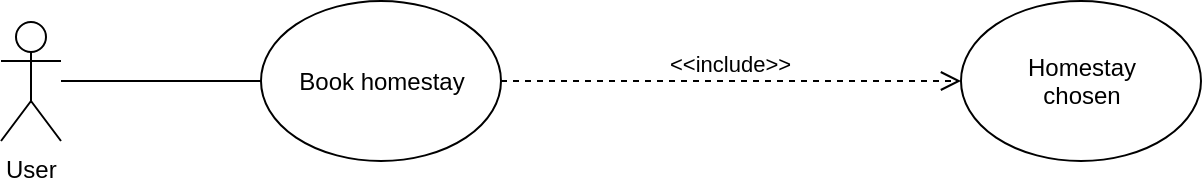
\includegraphics[width = 10cm, height = 1cm]{parts/Khoa/khoa_ui/book.png}
	\caption{Lược đồ use case của Module 5: Đặt phòng homestay}
\end{figure}
\begin{figure}[!h]
	\centering
	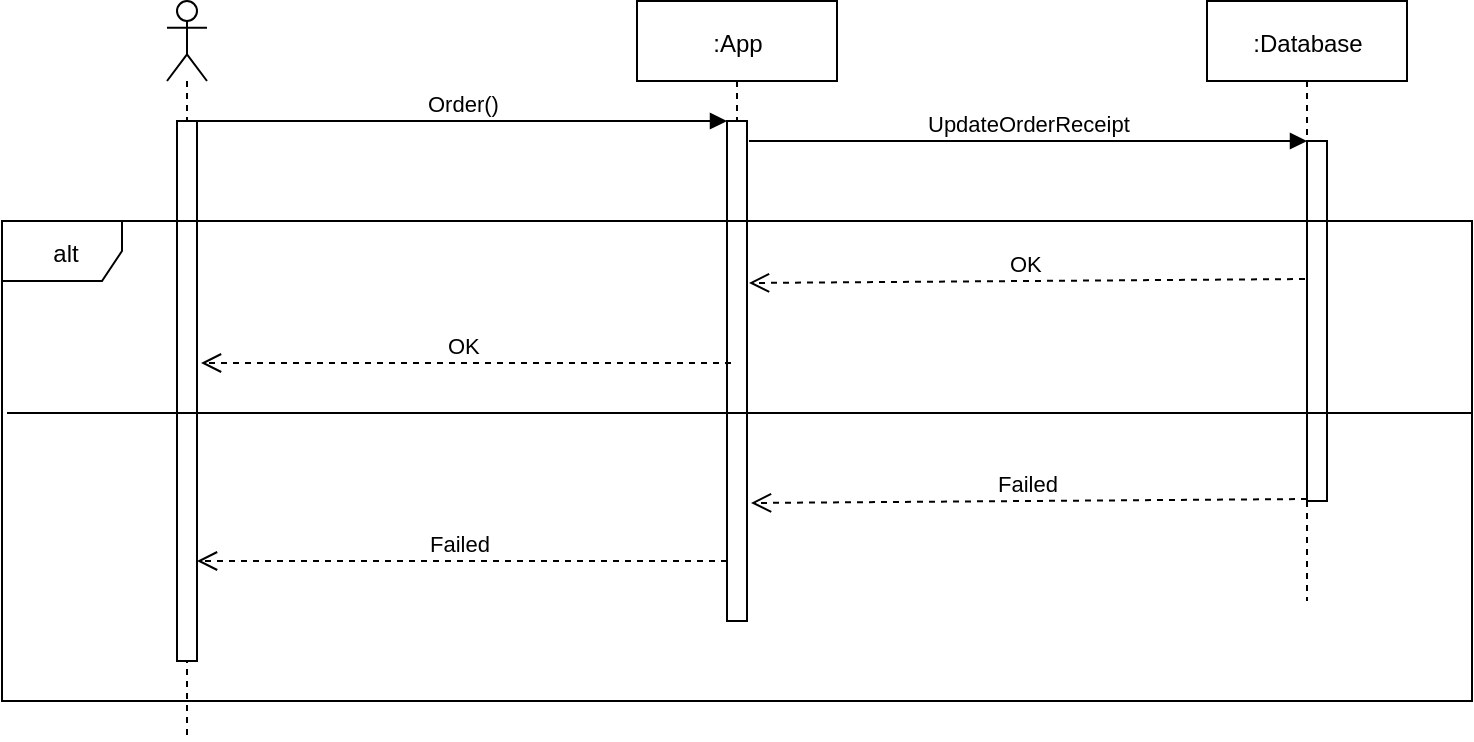
\includegraphics[width = 10cm, height = 6cm]{parts/Khoa/khoa_ui/khoa_order.png}
	\caption{Sequence diagram của Module 5: Tìm kiếm và lọc kết quả}
\end{figure}
\subsubsubsection{User story}
Sau khi chọn cho mình một homestay ưng ý, việc tiếp theo mà người dùng sẽ thực hiện chính là đặt phòng. Trang web sẽ yêu cầu người dùng nhập và kiểm tra một số thông tin quan trọng (và có thể xác minh nếu cần thiết). Nếu thành công, trang web sẽ thông báo và gửi thông báo đến người dùng. Nếu không thành công, trang web tự động thoát ra khỏi chế độ đặt phòng và người dùng phải làm lại 1 lần nữa.
\subsubsubsection{Mô tả các use case}
\begin{enumerate}[label=\textbf{(\alph*)}]
	\item \textbf{Usecase 3: Đặt phòng.}
	\begin{center}
		\begin{longtable}{ | l |p{10cm}|}
			\hline
			\textbf{Tên usecase} & Đặt phòng và thanh toán. \\ \hline
			\textbf{Người tương tác} & Người dùng ứng dụng. \\ \hline   
			\textbf{Mô tả} &  Người dùng đặt phòng homestay mà mình chọn và thanh toán.\\ \hline  
			\textbf{Người tạo:} \textit{Nguyễn Phan Đăng Khoa} & \textbf{Cập nhật lần cuối bởi:} \textit{Nguyễn Phan Đăng Khoa} \\ \hline
			\textbf{Ngày tạo:} \textit{22/03/2019} & \textbf{Lần cuối cập nhật:} \textit{30/03/2019} \\ \hline
			\textbf{Tiền điều kiện} &  Trước khi có thể 2 đặt phòng, người dùng phải chọn một trong các homestay mà mình đã tìm kiếm/lọc. \\ \hline 
			\textbf{Hậu điều kiện} &  Đặt phòng hoàn tất, mẫu ghi nhớ sẽ lưu vào tài khoản người dùng. \\ \hline 
			\textbf{Luồng cơ bản} & 
			\begin{enumerate}
				\item  Người dùng chọn vào nút "Đặt phòng".
				\item Một bản lịch sẽ hiện ra. Những ngày mà homestay không chấp thuận (đã có người ở, những ngày trước ngày đang đặt phòng,...) sẽ được gạch chéo. Người dùng có thể thay đổi ngày "Check in" và "Check out" nếu muốn. Sau khi hoàn tất chỉnh sửa, người dùng nhấn chọn nút "Tiếp theo".
				\item Người dùng xác nhận thông tin đặt chỗ. Các thông tin như ngày "Check in", ngày "Check out", số khách, số tiền, vị trí homestay sẽ được hiển thị. Người dùng kiểm tra và nhấn nút "Đặt ngay".
				\item Người dùng xác nhận thông tin liên hệ và thông tin tài khoản. Các thông tin như tên người đặt phòng, số điện thoại liên hệ, nơi cư trú sẽ được hiển thị. Người dùng xác  nhận và nhấn nút "Thanh toán".
				\item  Ở trang thanh toán, các lựa chọn như "Thẻ Quốc Tế", "Thẻ ATM Nội Địa" là các lựa chọn mà người dùng có thể thanh toán. Sau khi chọn, người dùng nhập thông tin cần thiết về tài khoản và nhấn nút xác nhận.
				\item Sau khi hoàn tất, trang web sẽ thông báo thành công và thông tin đặt phòng sẽ được lưu vào tài khoản người dùng.
			\end{enumerate} \\ \hline 
			\textbf{Luồng thay thế} & 
			\begin{itemize} 
				\item \textit{Luồng thay thế 1}
				\begin{enumerate}
					\item Tại bước 2:  Nếu sau khi chọn ngày xong, người dùng lại muốn đặt lại lịch, thì người dùng có thể nhấn nút "Đặt lại" để có thể chọn lại ngày "Check in" và "Check out".
					\item Tại bước 3: Nếu người dùng muốn thay đổi lại thông tin, người dùng có thể nhấn nút "Quay lại" để thay đổi các thông tin cần thiết.
					\item Tại bước 4: Nếu người dùng muốn thay đổi thông tin liên hệ thì có thể nhấn vào các khung thông tin đó và thay đổi thông tin liên hệ.
					\item Tại bước 6: Nếu không thành công, trang web sẽ báo lỗi và thanh toán sẽ không thực hiện.
				\end{enumerate}
			\end{itemize} \\ \hline 
			\textbf{Ngoại lệ}  & Không có \\
			\hline
		\end{longtable}
	\end{center}
\end{enumerate}
